\chapter{Introduction to Group}

\section{Introduction}

\begin{remark}
    What have we done so far: we have studied some \bred{objects} with some properties, and we have asked how can we operate in this object and preserve its property. 
\end{remark}

\begin{definition}[Group]\index{Group}\label{def:group}
    A \term{group} is a pair $(G, \cdot)$ where $G$ is a set and $\cdot$ is a binary operation on $G$ such that \[
        \begin{matrix}[cccc]
            \cdot & G \times G & \to     & G         \\
                  & (a, b)     & \mapsto & a \cdot b
        \end{matrix}
    \] such that \begin{listu}
        \item \textbf{Identity:} There exists an element $e \in G$ such that \[ e \cdot g = g \cdot e = a \quad \forall a \in G. \]
        \item \textbf{Inverse:} For every $g \in G$ there exists an element $h \in G$ such that \[ g \cdot h = h \cdot g = e. \]
        \item \textbf{Associativity:} For every $g, h, k \in G$ we have \[ g \cdot (h \cdot k) = (g \cdot h) \cdot k. \]
    \end{listu}
\end{definition}

\begin{definition}[Abelian Group]\index{Abelian Group}\label{def:abelian_group}
    A group $(G, \cdot)$ is called \term{abelian} if \[ g \cdot h = h \cdot g \quad \forall g, h \in G. \]

    This group is also called a \term{commutative group}.
\end{definition}

The term \textit{abelian} comes from the name of the Norwegian mathematician \href{https://en.wikipedia.org/wiki/Niels_Henrik_Abel}{Niels Henrik Abel}. He was the first to prove the impossibility of solving the general quintic equation in radicals. He also made important contributions to the study of elliptic functions, discovered Abelian functions, and many other important fields in mathematics.

\begin{example}
    We will consider the following ``toy"

    \begin{center}
        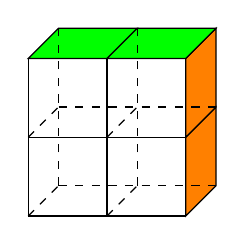
\begin{tikzpicture}
            \draw (0,0,0) -- (1,0,0) -- (1,1,0) -- (0,1,0) -- cycle;
            \draw (1,0,0) -- (2,0,0) -- (2,1,0) -- (1,1,0) -- cycle;
            \draw (0,1,0) -- (1,1,0) -- (1,2,0) -- (0,2,0) -- cycle;
            \draw (1,1,0) -- (2,1,0) -- (2,2,0) -- (1,2,0) -- cycle;

            \draw[fill=orange] (2,0,0) -- (2,0,-1) -- (2,1,-1) -- (2,1,0) -- cycle;
            \draw[fill=orange] (2,1,0) -- (2,1,-1) -- (2,2,-1) -- (2,2,0) -- cycle;

            \draw[fill=green] (0,2,0) -- (1,2,0) -- (1,2,-1) -- (0,2,-1) -- cycle;
            \draw[fill=green] (1,2,0) -- (2,2,0) -- (2,2,-1) -- (1,2,-1) -- cycle;

            % Dashed invisible lines
            \draw[dashed] (0,0,0) -- (0,0,-1);
            \draw[dashed] (1,0,0) -- (1,0,-1);
            \draw[dashed] (0,1,0) -- (0,1,-1);
            \draw[dashed] (1,1,0) -- (1,1,-1);
            \draw[dashed] (0,0,-1) -- (0,2,-1);
            \draw[dashed] (1,0,-1) -- (1,2,-1);
            \draw[dashed] (0,0,-1) -- (2,0,-1);
            \draw[dashed] (0,1,-1) -- (2,1,-1);
        \end{tikzpicture}

        The left side is red, the bottom is blue, and the back is yellow. 
    \end{center}

    We have $7$ operations \[
        V_1, V_2, H_1, H_2, V, H, R
    \] where \begin{listu}
        % TODO: add picture
        \item $V_1$ is the vertical flip of the first column
        \item $V_2$ is the vertical flip of the second column
        \item $H_1$ is the horizontal flip of the first row
        \item $H_2$ is the horizontal flip of the second row
        \item $V$ is the vertical flip of the whole cube
        \item $H$ is the horizontal flip of the whole cube
        \item $R$ is the rotation of the cube by $90^\circ$ around the vertical axis
    \end{listu}
    
    They satisfy \[
        {V_1}^2 = 1, {V_2}^2 = 1, {H_1}^2 = 1, {H_2}^2 = 1, V^2 = 1, H^2 = 1, R^4 = 1, 
    \]

    However, we have redundancies: \begin{listu}
        \item $V_1 V_2 = V_2 V_1 = V$
        \item $H_1 H_2 = H_2 H_1 = H$
        \item $V_1 H_1 = H_1 V_1 = R$
        \item $H_2 H_1 V_2 V_1 = R^2$
        \item $R^3 V_1 R = R^{-1} V_1 R = H_1$ 
        \item \dots
    \end{listu}

    We can flatten the cube into
    \begin{center} \begin{tabular}{c|c} 1 & 2 \\ \hline 3 & 4 \end{tabular} \end{center}

    Then, \begin{listu}
        \item $V_1 = (1, 4)$ 
        \begin{center} 
            \begin{tabular}{c|c} 1 & 2 \\ \hline 4 & 3 \end{tabular}
            \quad$\xrightarrow{V_1}$\quad
            \begin{tabular}{c|c} 4 & 2 \\ \hline 1 & 3 \end{tabular} 
        \end{center}

        \item $V_2 = (2, 3)$
        \begin{center} 
            \begin{tabular}{c|c} 1 & 2 \\ \hline 4 & 3 \end{tabular}
            \quad$\xrightarrow{V_2}$\quad
            \begin{tabular}{c|c} 1 & 3 \\ \hline 4 & 2 \end{tabular}
        \end{center}

        \item $H_1 = (1, 2)$
        \begin{center} 
            \begin{tabular}{c|c} 1 & 2 \\ \hline 4 & 3 \end{tabular}
            \quad$\xrightarrow{H_1}$\quad
            \begin{tabular}{c|c} 4 & 3 \\ \hline 1 & 2 \end{tabular}
        \end{center}

        \item $H_2 = (3, 4)$
        \begin{center} 
            \begin{tabular}{c|c} 1 & 2 \\ \hline 4 & 3 \end{tabular}
            \quad$\xrightarrow{H_2}$\quad
            \begin{tabular}{c|c} 1 & 2 \\ \hline 3 & 4 \end{tabular}
        \end{center}

        % \item $V = (1, 4)(2, 3)$

        \item $R = (1, 2, 3, 4)$
        \begin{center} 
            \begin{tabular}{c|c} 1 & 2 \\ \hline 4 & 3 \end{tabular}
            \quad$\xrightarrow{R}$\quad
            \begin{tabular}{c|c} 4 & 1 \\ \hline 3 & 2 \end{tabular}
        \end{center}
    \end{listu}

    We can verify that \[
        (1, 2, 3, 4) = (3, 4)(1, 4)(1, 2),
    \] which proposes that \[
        R = H_2 \circ V_1 \circ H_1
    \]

    % TODO: add picture
\end{example}

We have a group that is the one generator by the operations of the `toy` above. We have two models to understand the group: \begin{listo}
    \item The complete toy 
    \item The location code
\end{listo} What we have seen is that these two models are codify information in different ways. We can generate a map of the potential positions. 

% TODO: image

\begin{center}
    \includegraphics[width=0.55\linewidth]{figures/rubics-cube-1.png}
\end{center}

If we only allow $H_1, V_1, H_2, V_2$, then the locations are believable. The group they generate is $S_4$. 